\section{mesh}

\subsection{Mesh type}

Dans un premier temps, pour réussir le travail que l’on m’a demandé, il a été nécessaire de connaître les contraintes imposées par le code pour chaque maillage.\\
Il a aussi été primordial de me documenter sur les différents maillages liés à des problèmes aérodynamiques.


\subsubsection{Généralité maillage}

Il existe différentes catégories de maillages. Ces différents types de maillages peuvent être associables et ils ont chacun des avantages et des inconvénients. Dans cette partie on détaillera les différents maillages en exposant leurs caractéristiques.\\

Les maillages cartésiens sont des maillages orthogonaux. Ils sont construits à partir de lignes à x, y constants en 2D et à x,y,z constants en 3D. Il seront alors composés de quadrangles en 2D et d'hexaèdres en 3D. Ce type de maillage à l'avantage d'être simple à construire et il permet l'utilisation de schémas numériques à ordre élevé lors de calculs en différence finie. L'inconvénient majeur de ce maillage est qu'il n'est pas adaptable pour des géométries courbés.\\
On retrouve ce type de maillage lors de calculs pour les "frontières immergées" où l'on ne prend pas en compte l'objet pour mailler le domaine de calcul.\\

Le maillage structuré en 2D (i,j) ou 3D (i,j,k) est un maillage cartésien qui a été déformé. Comme pour le maillage cartésien il sera alors composé de quadrangles ou d'hexaèdres selon sa dimension. On peut identifier facilement les cellules de ce maillage à l'aide des indices des nœuds qui le compose. En 2D les indices seront des doublets et en 3D se sera des triplets.
Étant similaire au maillage cartésien, il a les mêmes inconvénients. Il est incapable de représenter des géométries complexes comme des chambres de combustion comprenant des trous ou des inclusions.\\
% la difficulté à donner un caractère local à l’adaptation qui se propage dans toutes les directions principales du maillage, comme le montre la figure 1.1.\\
Il est tout de même possible d'adapter un maillage structuré sur des géométries complexes en utilisant la méthode de maillage multibloc. En décomposant le domaine de calcul en plusieurs sous-domaines, appelés blocs. Chaque sous domaine est maillé indépendamment des autres. Cela permet d'adapter le maillage à la géométrie de l'objet.\\

Le dernier type de maillage présenté est le maillage non-structuré. Pour des géométries extrêmement complexes on a recours à ce genre de maillage. La génération d'un maillage pour s'adapter à une géométrie est beaucoup plus simple en non-structuré qu’en structuré. Les éléments qui le composent sont en général des triangles en 2D et des tétraèdres en 3D. Ce maillage est généré arbitrairement et sans contraintes pour la disposition des mailles. Il permet de conserver une bonne qualité des éléments pour les géométries complexes.\\
En revanche il est très couteux en nombres d'éléments et il peut engendrer des erreurs numériques plus importantes qu’un maillage structuré.\\
Il existe un dernier type de maillage qui est l’hybride. Il est la combinaison d'éléments triangulaires et de quadrangles en 2D, les mailles seront des tétraèdres et des hexaèdres en 3D.\\
Ce maillage a les avantages des maillages structurés et non-structurés en réduisant les erreurs numériques. Il est difficile à générer notamment au niveaux des liaisons entre les deux types de maillages.


%Pour mailler certaines géométries très complexes, le recours aux maillages non-structurés est une solution. La génération d’un maillage initial s’adaptant à une géométrie complexe est beaucoup plus simple qu’en structuré. De plus, l’utilisation de maillages non-structurés permet de limiter le raffinement à une zone locale dans le cas général comme expliqué dans le rapport technique de Dervieux et Désidéri [27]. Cependant, l’inconvénient par rapport aux maillages structurés est le coût du stockage de la topologie du maillage. Par exemple, pour une méthode de type « volumes finis » avec les valeurs définies aux centres des cellules, il est en effet nécessaire de stocker une table de connectivité donnant les indices des cellules gauche et droite pour chacune des interfaces du maillage et des tableaux donnant les indices des nœuds qui composent chaque interface et chaque cellule. Ces maillages sont généralement composés de triangles en 2D et de tétraèdres, prismes, pyramides et hexaèdres en 3D. La figure 1.2, extraite de l’article de Dobrzynski et Frey [32], présente un maillage adapté à la prise en compte d’un choc plan dans le domaine de calcul. On y voit bien que le raffinement est localisé au niveau du choc et ne se propage pas au reste du domaine.

\subsection{GMSH}
Le second logiciel est GMSH développé par GMESH de Christophe Geuzaine et Jean-François Remacle de l'université de Louvain. Il a été choisi parce qu'il est possible d'écrire des scripts en Python. De plus, GMSH est un logiciel libre et évolutif. Il sera possible de demander au développeur d'inclure de nouvelles fonctionnalités pour le CEA/CESTA.

Le travail effectué avec GMSH s'est fait sur un environnement linux. Dans un premier temps, il a fallu installer une machine virtuelle pour obtenir linux sur ma machine. Travailler avec ce nouveau bureau m'as permis de me familiariser avec ce système d'exploitation que j'ai utilisé par la suite au CEA.

Le travail effectué avec GMSH s'est fait entièrement sur la machine virtuelle. Ce logiciel de maillage a des avantages et des inconvénients. GMSH est performant pour réaliser des maillages non structurés. Il possède également des capacités en maillage structuré que nous souhaitons évaluer dans le cadre de cette étude.\\
De plus, ce logiciel est utilisable de différentes façons: on peut soit réaliser ses maillages en utilisant l'interface interactive, soit en écrivant un script via des éditeurs de texte ou bien en codant le maillage directement. Chaque méthode est utilisée pour réaliser les différents cas. La version que j'ai utilisée est GMSH 4.5.6.

La méthode interactive permet de produire les géométries et les maillages facilement. On commence par choisir quel type de ressource utiliser pour la création de la géométrie. Nous avons adopté le modeleur basé sur "OpenCascade".\\
La création d'objet en mode interactif se fait en sélectionnant les différentes options et en rentrant les paramètres directement sur l'interface du logiciel comme pour les coordonnées de points par exemple. Néanmoins avec cette méthode nous ne pouvons pas paramétrer les géométries ni le maillage.

La seconde utilisation se fait avec un script, au sein d'un éditeur. Cette méthode est intéressante car elle permet de définir des paramètres comme les rayons des cercles ou la longueur d'un rectangle. De plus, en écrivant son fichier texte, à la moindre erreur nous pouvons la rectifier rapidement.\\
Cette méthode reste intéressante car le langage de description est utilisé pour d'autres logiciels notamment "Openfoam" pour la mécanique des fluides.

La dernière méthode est de développer un code en utilisant l'API GMSH pour réaliser son maillage et sa géométrie. Plusieurs langages sont disponibles comme le C ou le C++, mais nous avons utilisé la langage Python.\\
Pour développer mes codes j'utilise un éditeur, "VScode". Utiliser un éditeur permet d'avoir plus de clarté que lorsqu'on travaille sur la console.\\
En utilisant le langage Python, on peut paramétrer son maillage et la géométrie facilement, il suffit de renseigner les différents arguments. Contrairement à l'utilisation de script nous pouvons utiliser les librairies et les fonctionnalités que nous offre le code Python. Il y a un le fichier python où toutes les commandes sont documentées pour générer les modèles que l'on souhaite, ce qui apporte une aide importante.

\subsubsection{H2-B}

Pour illustrer le logiciel Gmsh je décide de réaliser un maillage sur un missile balistique le HB-2.\\
Ce maillage est réalisé à l'aide d'un code python.\\
Dans un premier temps j'importe la géométrie de l'objet. Cette entité est symétrique et peut donc être simulée en prenant en compte uniquement la moitié de la géométrie, ce qui permettra de diminuer le nombre de mailles ainsi que le nombre de blocs. Je supprime alors les différentes droites et points de la partie inférieure pour n'utiliser que la moitié du profil.\\
Le domaine de calcul est représenté sur la figure suivante, l'amont a été réalisé en faisant un agrandissement de la tête du HB-2.\\
Je le découpe en différents blocs choisis arbitrairement.

\begin{figure}[H]
\begin{center}
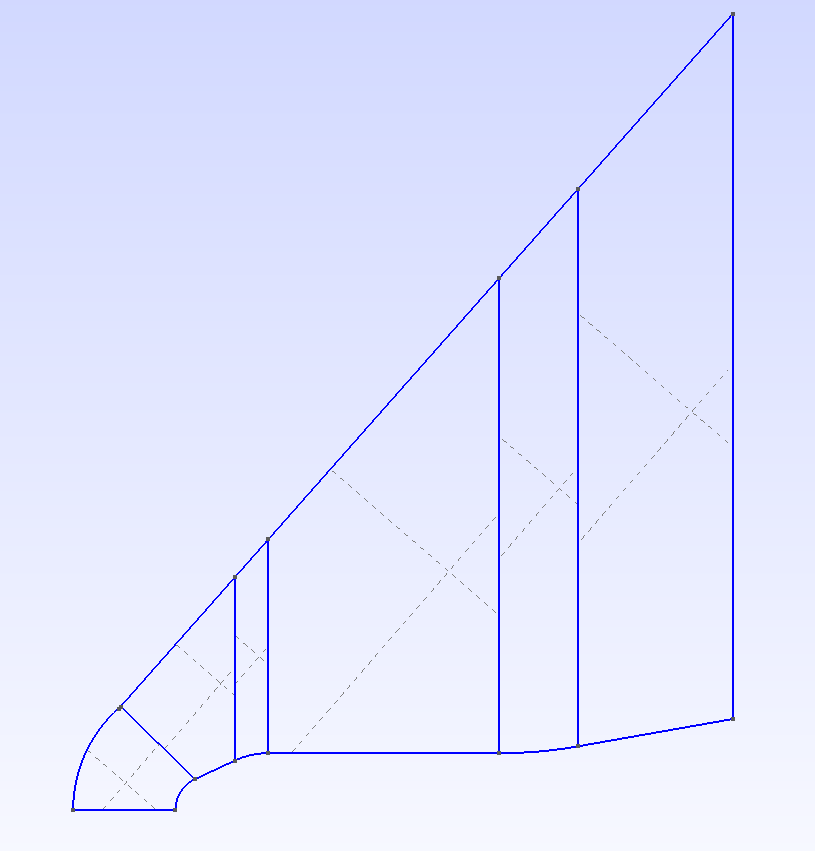
\includegraphics[width=0.5\textwidth]{chapter1_introduction/pictures/gmsh/hb2_geo.png}
\caption{Géométrie HB-2}
\end{center}
\end{figure}

Par la suite je crée les différentes surfaces sur chaque bloc. On veut obtenir un maillage structuré. Il est nécessaire de définir des surfaces à quatre côtés. Si les surfaces ont plus de quatre cotés il sera alors impossible d'utiliser les fonctions dites ‘transfinite’ pour produire un maillage structuré.\\
J'utilise les fonctions 'transfinite curve' sur les différentes droites pour définir le nombre de discrétisations et la progression géométrique des mailles.\\
Pour finir, il faut définir les conditions aux limites, l'amont qui est l'intérieur du domaine, l'aval qui est la sortie, la paroi qui représente l'objet et la droite en amont du HB-2 est définie en tant que symétrie à l'aide des fonctions 'physical line'.\\
Le maillage réalisé et présenté sur les figures suivantes.

Le HB-2 n'est pas très compliqué à mailler,  le domaine est adapté à la géométrie pour obtenir un maillage orthogonal à la paroi.


\begin{figure}[H]
\begin{center}
\begin{subfigure}{0.5\textwidth}
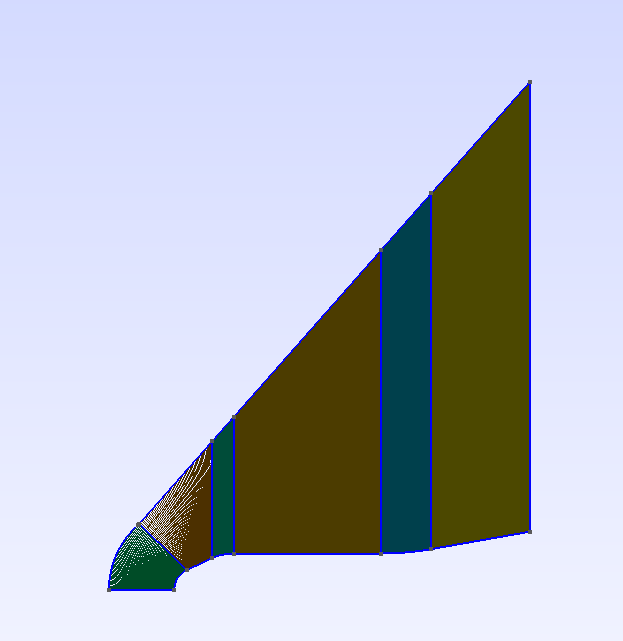
\includegraphics[width=\textwidth]{chapter1_introduction/pictures/gmsh/hb2_mesh1.png}
\end{subfigure}
\begin{subfigure}{0.5\textwidth}
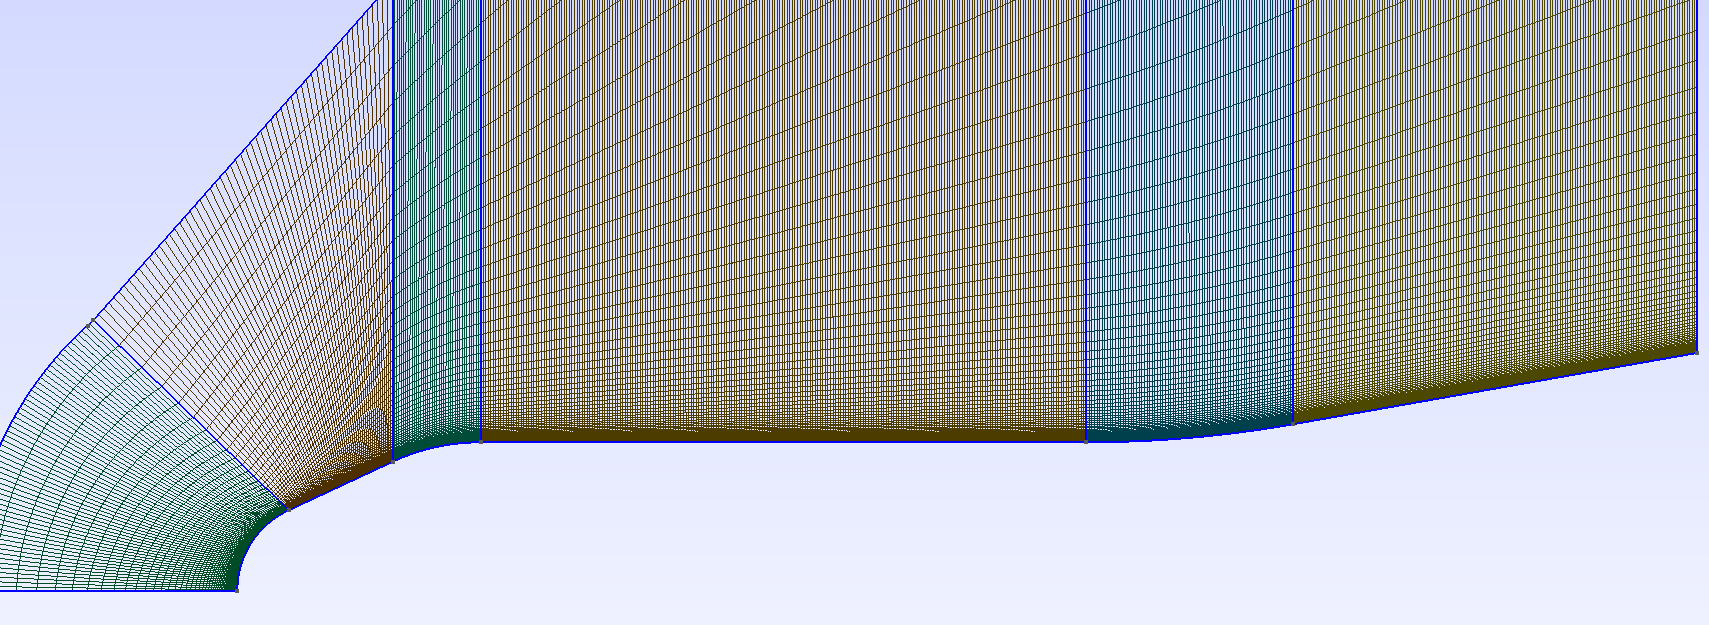
\includegraphics[width=\textwidth]{chapter1_introduction/pictures/gmsh/hb2_mesh2.png}
\end{subfigure}
\begin{subfigure}{0.5\textwidth}
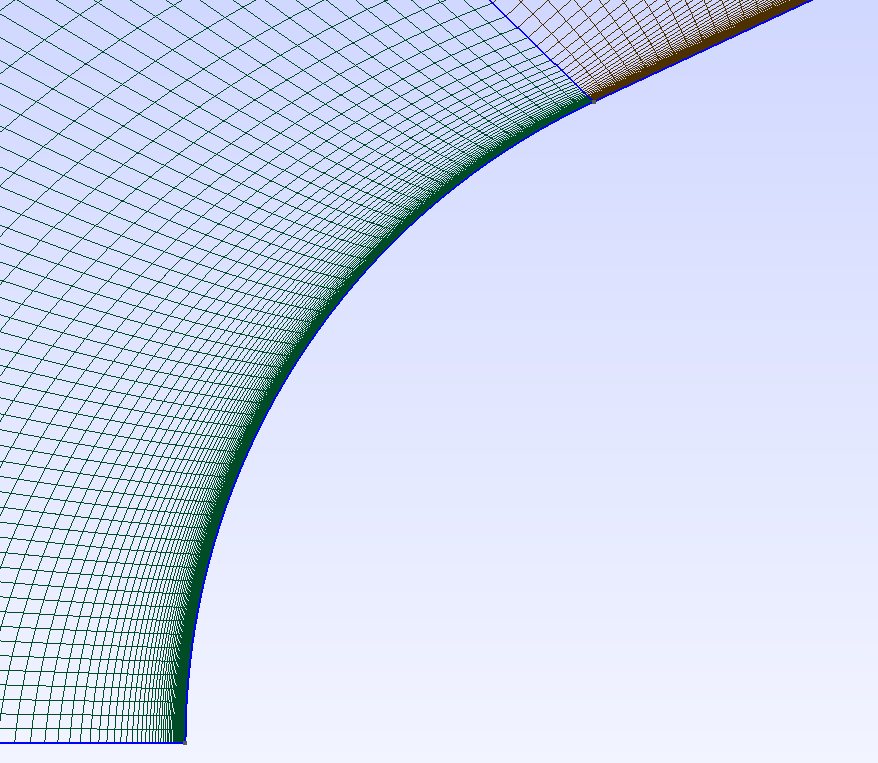
\includegraphics[width=\textwidth]{chapter1_introduction/pictures/gmsh/hb2_mesh3.png}
\end{subfigure}
\caption{Maillage final du HB-2}
\end{center}
\end{figure}
\newpage
\subsubsection{Qualité du maillage}

Une fois le maillage terminé, nous pouvons regarder sa qualité à l'aide de trois critères qui sont 'Gamma',  'SICN' et 'SIGE. Ce sont les seuls critères que le logiciel propose. On les calcule respectivement de la façon suivante:


\begin{equation}
    \gamma = \frac{r_{ci}}{r_{cc}}
\end{equation}

\begin{equation}
    \eta = \frac{V^{\frac{2}{3}}}{\sum l_a^2}
\end{equation}

\begin{equation}
    \epsilon = \frac{minl_a}{maxl_a}
\end{equation}

V représente le volume ou l'aire de l'élément 3D ou 2D, $l_a$ est la longueur d'une arête, $r_{cc}$ est le rayon de la sphère circonscrit en 3D et du cercle circonscrit en 2D, $r_{ci}$ est le rayon de la sphère ou du cercle inscrit en 3D ou en 2D.

Pour le maillage structuré je m'intéresse à deux critères en particulier le 'Gamma' est le 'SIGE'.\\
Plus la valeur de 'Gamma' est proche de 1, plus la qualité du maillage est bonne, si le maillage contient des valeurs avec un faible gamma alors les éléments sont dits distordus et ils vont détériorer les résultats des simulations. Les valeurs pour ce critère sont assez bonnes dans l'ensemble, ils sont compris entre [0.42,1], avec les valeurs les plus basses dans le champ lointain.

Le critère 'SIGE' correspond à la longueur minimum d'une arête d'un élément divisée par la longueur maximale d'une arête du même élément. Après normalisation, plus le critère est proche de 1, meilleur est la qualité du maillage qui permettra d'éviter des erreurs ou des difficultés lors des calculs numériques.

Les valeurs moyennes pour ces deux critères sont répertoriées dans le tableau suivant.

\begin{figure}[H]
\begin{center}
\begin{subfigure}{0.48\textwidth}
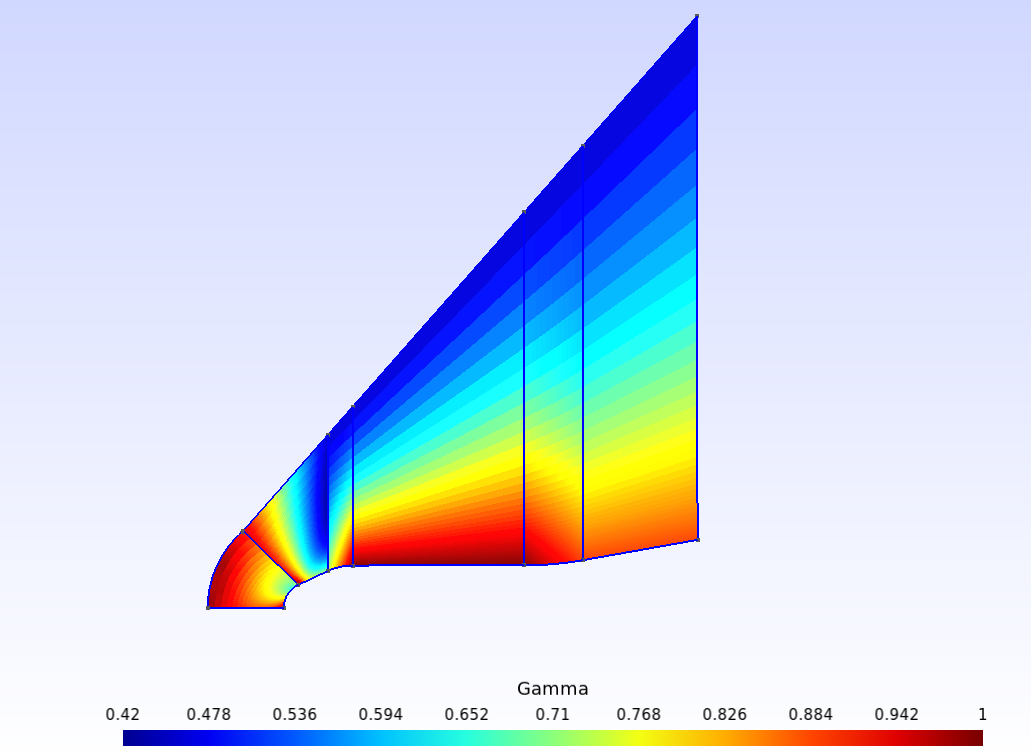
\includegraphics[width=\textwidth]{chapter1_introduction/pictures/gmsh/gamma.png}
\end{subfigure}
\begin{subfigure}{0.48\textwidth}
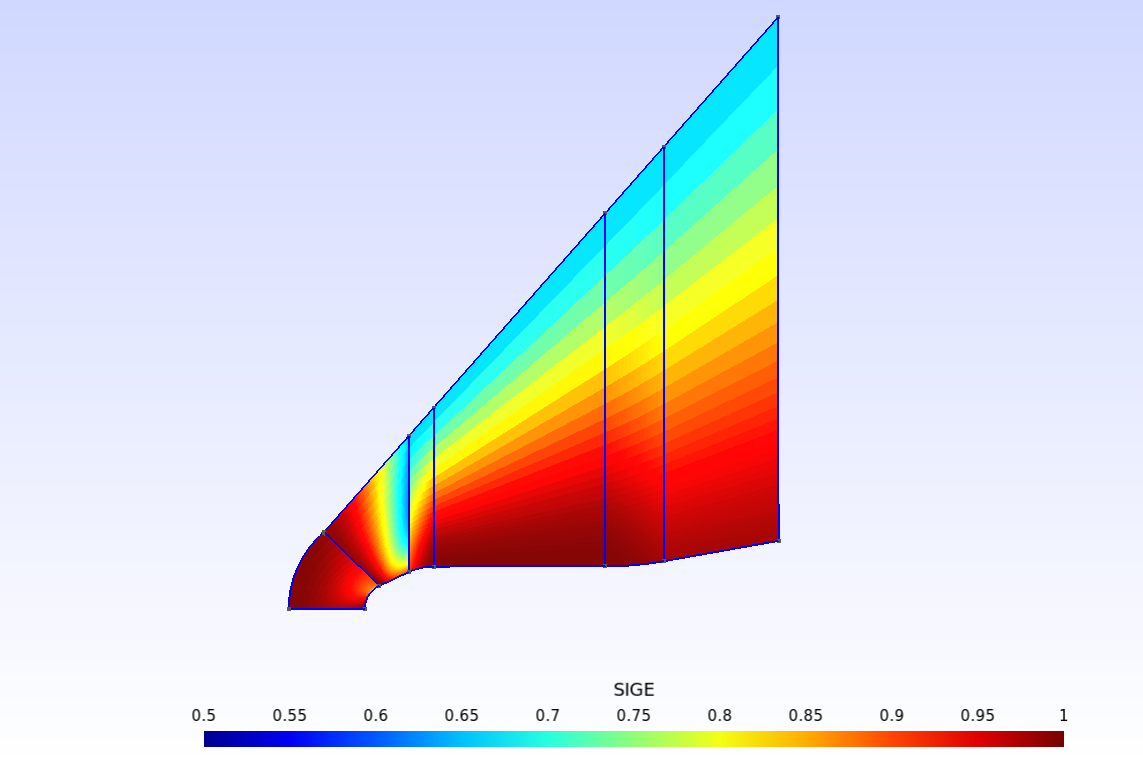
\includegraphics[width=\textwidth]{chapter1_introduction/pictures/gmsh/critere1.png}
\end{subfigure}
\caption{Critére Gamma et SIGE}
\end{center}
\end{figure}

\begin{center}
\begin{tabular}{|c|c|}%3 pour trois colonnes
\hline%ligne horizontale
 Gamma& 0.84 \\%valeur des cases sur une horizontale
\hline
SIGE  &0.92 \\
\hline
\end{tabular}
\captionof{table}{Valeur moyenne de Gamma et SIGE}
\end{center}

\subsection{ICEM}

Le but de mon stage est d'évaluer trois mailleurs entre eux. Lors des trois prochains chapitres nous détaillerons les environnements de travail de chaque mailleur, nous présenterons la réalisation d'un maillage sur logiciel ainsi que leurs critères de qualité. Pour évaluer au mieux ces outils, chaque maillage a été réalisé avec chacun des mailleurs. D’autres cas de comparaison sont aussi en annexe.\\
On commencera par le logiciel actuellement utilisé au sein de CEA/CESTA: ICEM CFD.\\

Le travail réalisé avec ICEM CFD s'est fait sur deux environnements différents. Le début du stage étant en télétravail, j'ai commencé par utiliser ce logiciel sur un environnement Windows.\\
Dès que j'ai pu retourner travailler sur le centre, la suite des travaux sur ICEM s'est faite sur un environnement linux. La version utilisée est la 19.2.\\

ICEM CFD est un mailleur proposé par l'éditeur ANSYS. Ce logiciel de maillage est extrêmement performant pour faire des maillages structurés et non-structurés, que ce soit en deux dimensions ou en trois dimensions.\\
La réalisation de maillage réglé en 2D et 3D se fait essentiellement à l'aide de la méthode multibloc pour obtenir une qualité de maillage élevée.\\
Avec ce logiciel il est facile de mailler des géométries simples pour réaliser un maillage multibloc structuré. Si les géométries deviennent plus complexes on doit employer des méthodes spécifiques aux problèmes avec plusieurs options implémentées au logiciel.\\

Je l‘ai utilisé de façon interactive. C'est à dire que l’on sélectionne les différentes options proposées par le logiciel pour réaliser le maillage mais aussi les géométries si on le souhaite. Cela permet de garder un visuel de la conception du maillage et du blocking réalisé.\\

L'utilisation de ICEM CFD est très difficile, surtout pour la réalisation de maillage multibloc structuré.\\
Pour réaliser un maillage conforme qui soit adapté à la géométrie, il faut procéder en plusieurs étapes et les réaliser dans un ordre bien précis, détaillé à travers l'exemple qui va suivre.\\
De plus pour des géométries en trois dimensions le blocking peut devenir compliqué à produire, il y aura énormément de blocs. Il faut alors réussir à visualiser la subdivision des différents blocs, adapter la géométrie des blocs, bien utiliser les fonctionnalités au risque de ne pas obtenir un maillage structuré.


\section{ Sphère-cône}

L'exemple pris pour le logiciel ICEM CFD est une géométrie composée d'une sphère et d'un cône, où je vais mailler la partie solide de l'objet ainsi que le domaine de calcul. La partie solide comprend une extrusion de matière d'un cône sphère en son centre.\\
Pour construire ce maillage, je commence par importer le fichier Step, qui un fichier de géométrie, comprenant le domaine de calcul ainsi que le solide.\\

Avec ce logiciel il est nécessaire de définir les conditions aux limites dès le début. Je commence par nommer les différentes parties comme l'amont et la paroi.


\begin{figure}[H]
\begin{center}
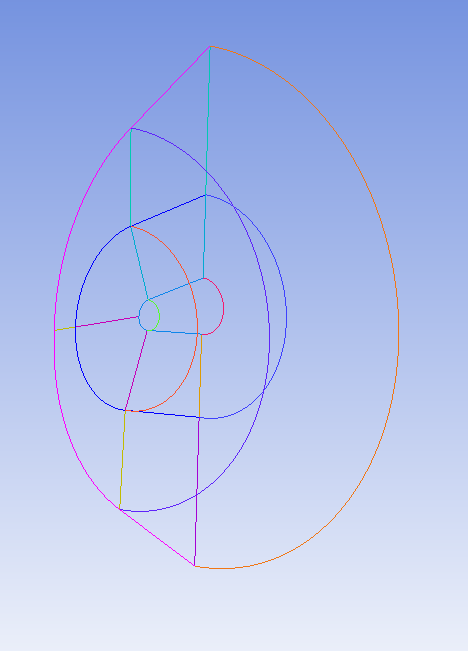
\includegraphics[width=0.45\textwidth]{chapter1_introduction/pictures/icem/castest_fluid_solid/geo1.PNG}
\caption{Géométrie sphère-cône}
\end{center}
\end{figure}

Pour avoir un maillage multibloc avec ICEM, je doi définir un bloc principal qui prend en compte l'intégralité de la géométrie importée, c'est à dire le domaine et l'entité géométrique.\\
Le domaine étant un cône sphère comme la géométrie, je décide d'utiliser la fonction ‘ogird’ pour découper le bloc principal. Cette fonction permet de créer une prézone autour de l'objet en définissant de nouveaux blocs autour de la géométrie.\\

Cette fonction est utilisée à deux reprises, une première fois pour la partie solide et une seconde fois pour la partie fluide.\\

Avec ICEM, il faut faire la différence entre les points, les sommets topologiques, les courbes et les arêtes. Les points et les courbes sont définies par les géométries alors que les sommets topologiques et les arêtes sont définies par la topologie. Il faut associer les courbes et les arêtes qui vont de pair et faire de même entre les sommets topologiques et les points. Une fois que les différentes associations sont faites, je dois supprimer le bloc central qui correspond à l'extrusion de matière.\\



\begin{figure}[H]
\begin{center}
\begin{subfigure}{0.5\textwidth}
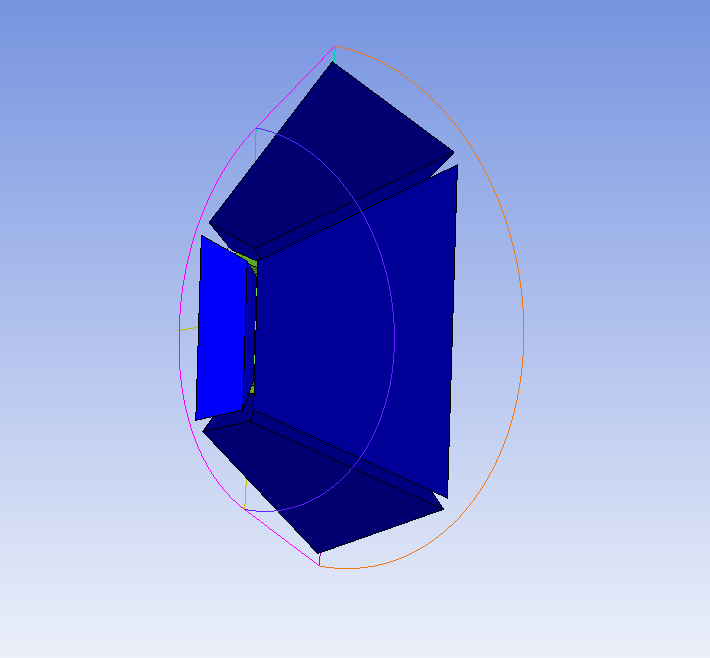
\includegraphics[width=\textwidth]{chapter1_introduction/pictures/icem/castest_fluid_solid/blk1.PNG}
\label{fig:subim1}
\end{subfigure}
\begin{subfigure}{0.5\textwidth}
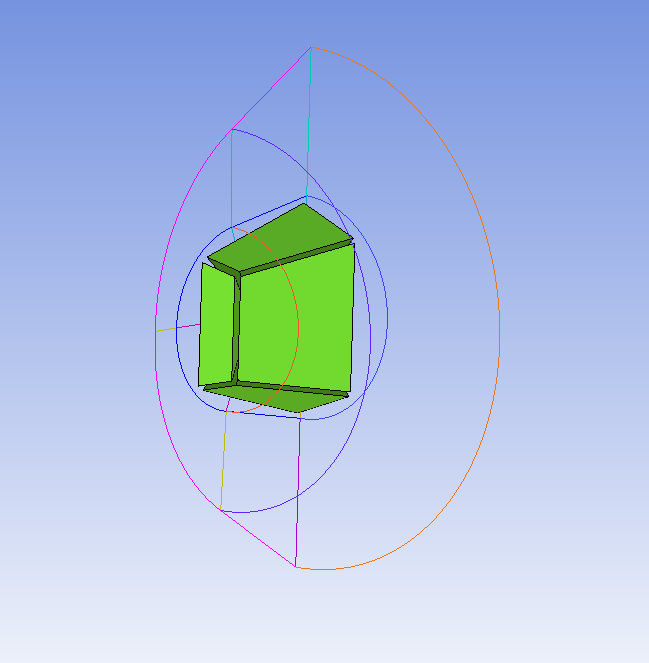
\includegraphics[width=\textwidth]{chapter1_introduction/pictures/icem/castest_fluid_solid/blk2.PNG}
\label{fig:subim2}
\end{subfigure}
\caption{Blocking sphère-cône}
\label{fig:image2}
\end{center}
\end{figure}

Pour finir il faut discrétiser chaque côté avec les fonctions de "sizing". Cette fonction a plusieurs paramètres qui permettent d’introduire du biais si on le souhaite. Il y a le "spacing 1" qui représente la taille de la première maille et le "spacing 2" qui est la taille de la dernière maille sur une courbe.\\
Pour savoir quelle est la première et la dernière maille d’une courbe il y a une flèche qui indique la direction du biais.\\

Pour faire varier le biais, il y a le "ratio 1" et le "ratio 2", que l’on augmente ou diminue pour avoir une progression du maillage.\\
De plus, il y a des fonctions utiles dans ICEM que nous utilisons comme celle qui permet d’avoir la même taille de maille d’un bloc à un autre, pour ne pas avoir de différence de maille inter-bloc.

\begin{figure}[H]
\begin{center}
\begin{subfigure}{0.6\textwidth}
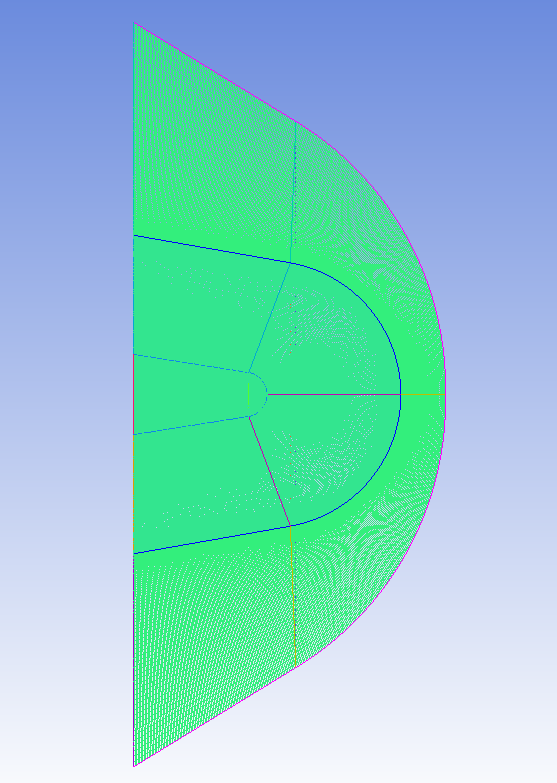
\includegraphics[width=\textwidth]{chapter1_introduction/pictures/icem/castest_fluid_solid/mesh1.PNG}
\label{fig:subim1}
\end{subfigure}
\begin{subfigure}{0.6\textwidth}
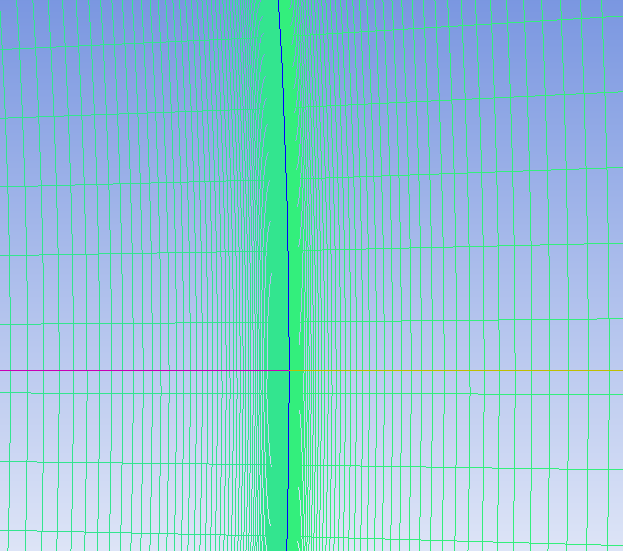
\includegraphics[width=\textwidth]{chapter1_introduction/pictures/icem/castest_fluid_solid/mesh2.PNG}
\label{fig:subim2}
\end{subfigure}
\caption{Maillage final du sphère-cône}
\label{fig:image2}
\end{center}
\end{figure}

\section{ Qualité du maillage}

On peut regarder la qualité d’un maillage à l'aide de certains paramètres. Pour des maillages composés exclusivement d'hexaèdres, les trois principaux critères de qualité sont le déterminant, la distorsion et l'angle.\\
J'ai choisi de regarder deux de ces éléments avec ICEM: le déterminant et l'angle.\\

Le déterminant peut être calculé pour des éléments linéaires hexaédriques, quads et pyramidaux. Sa valeur est calculée à chaque nœud de chaque élément.\\
La valeur du déterminant est comprise entre [0,1]. Un élément du maillage est dit régulier si sa valeur est proche de 1, et il sera dégénéré s’il est proche de 0. Si la valeur est inférieure à 0 alors les éléments sont dits inversés et pourraient compromettre les résultats du calcul numérique.\\
Pour la plupart des solveurs, il faut une valeur supérieure à 0,1. Nos valeurs sont comprises entre [0.8,1], ainsi le maillage sera utilisable par les différents solveurs.


\begin{figure}[H]
\begin{center}
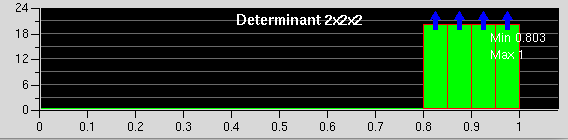
\includegraphics[width=\textwidth]{chapter1_introduction/pictures/icem/castest_fluid_solid/det2.PNG}
\caption{Déterminant 2x2x2}
\end{center}
\end{figure}




L'angle représente les valeurs des angles internes des faces de chaque élément. Ces valeurs sont comprises entre entre 0 et 90 degrés.\\
Ce critère permet de connaître l'aplatissement des cellules qui composent le maillage, plus l'angle est petit et plus la maille sera aplatie et pourra compliquer le calcul par la suite.\\
Pour que le maillage soit utilisable sur les solveurs il faut des valeurs d’angles comprises entre 18 degrés et 90 degrés.


\begin{figure}[H]
\begin{center}
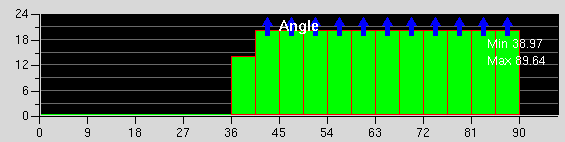
\includegraphics[width=\textwidth]{chapter1_introduction/pictures/icem/castest_fluid_solid/angle.PNG}
\caption{Angle}
\end{center}
\end{figure}
